\documentclass[12pt]{article}

\usepackage{amsmath}
\usepackage{amssymb}
\usepackage{amssymb}
\usepackage{graphicx}


\def\C{{\mathbb C}}
\def\E{{\mathbb E}}
\def\N{{\mathbb N}}
\def\Q{{\mathbb Q}}
\def\R{{\mathbb R}}
\def\T{{\mathbb T}}
\def\Z{{\mathbb Z}}

\begin{document}

\centerline{\large \bf Homework 1: due April 18, 2016}
\bigskip

\bigskip
\noindent
{\bf Problem 1:} 
Show that two random vectors in high dimensions are almost orthogonal.

{\em Note: In your theorem you need to formalize what ``almost orthogonal'' means (what it means will come
out of your proof). You first need to select a probability distribution of your choice and apply
an appropriate concentration inequality (but keep in mind that if e.g.\ $x$ and $y$ are Gaussian random
vectors, then the entries of the inner product $\langle x, y \rangle$ are no longer Gaussian).}

\bigskip
\noindent
{\bf Problem 2:} Consider the following setup. Given a square of side length 1, we place four circles
in the square as depicted in Figure~\ref{fig1} (each of the gray circles has radius 1/4). We now place a circle
at the center of the square (the blue circle in Figure~\ref{fig1}) such that this circle in the middle touches each of 
the four identical circles. Let $r$ denote the radius of the blue circle. 

\begin{figure}[ht!]
\begin{center}
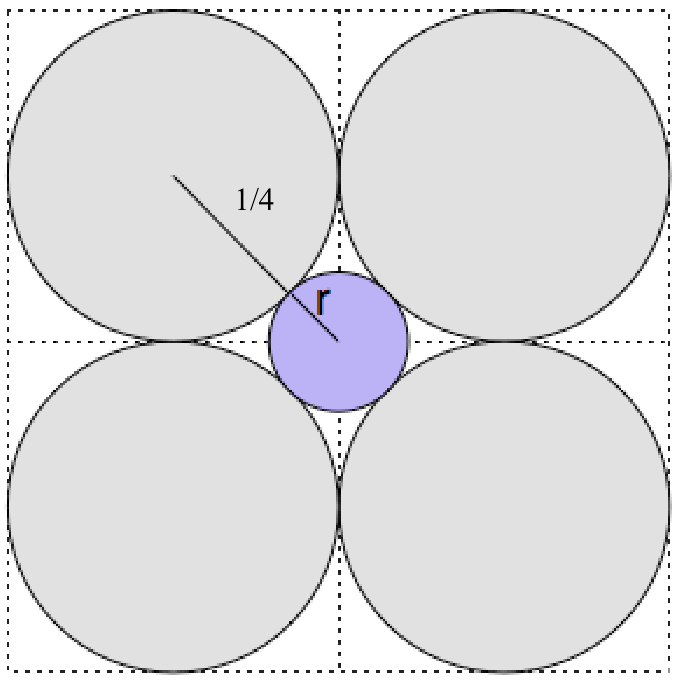
\includegraphics[width=40mm]{4circles1}
\caption{4 circles}
\label{fig1}
\end{center}
\end{figure}

We can do something analogous in three dimensions, see Figure~\ref{fig2}. We place eight spheres of 
radius 1/4 inside a cube of side length 1, and put a (blue) sphere in the middle such that it touches
all eight (gray) spheres.

\begin{figure}[ht!]
\begin{center}
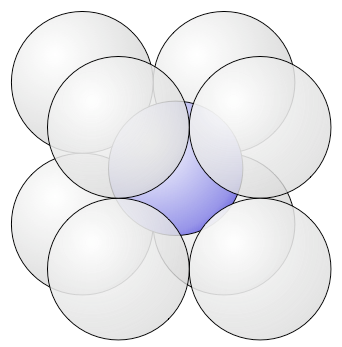
\includegraphics[width=40mm]{8spheres}
\caption{8 spheres}
\label{fig2}
\end{center}
\end{figure}

In four dimensions we can arrange 16 hyperspheres of radius 1/4 inside a hypercube of side length 1 and place a
hypersphere in the middle, so that this hypersphere all the other 16 hyperspheres.

Obviously we can do this for increasing dimension $d$. What happens with the blue hypersphere in the middle as
$d$ increases?
Will it shrink? Will it be of constant size? Will it grow outside the hypercube?

(Hint: Check the diameter of the blue hypersphere in comparison to the sidelength of the cube as $d$ increases. 
This is actually not difficult to compute, it may sound more complicated than it is).

\bigskip
\noindent
{\bf Problem 3:} 
Show that for every fixed dimension reduction matrix $A$ of size $k \times d$ with $k < d$, there exists vectors
$x,y \in \R^d$ such that the distance  $\|Ax-Ay\|$ (no matter which norm we use) is vastly different from
$\|x-y\|$.

\bigskip
\noindent
{\bf Problem 4:} 
The Yale Face Database contains images from various individuals in different poses and under different lighting
conditions. Some of the images are stored in the file {\tt SomeYaleFaces.mat}.

Load this file into Matlab. The variable {\tt X} is a matrix of size $1024 \times 2414$. Each column of {\tt X} 
is an image of size $32 \times 32$ (in vectorized form). 
The 2414 columns are images of 38 different persons in about 64 poses each.
You can easily covert the $k$-th column of {\tt X} back 
to an image via the commands \\
{\tt xk = X(:,k);} 
{\tt xk = reshape(xk,32,32);}  \\
The command \\ {\tt imagesc(x1); colormap(gray);} \\
will display the image.

You can conveniently display multiple images if you want with the file {\tt showfaces.m}.

We want to compare three dimension reduction methods by comparing how well distances between the differen images
are preserved: (i) Johnson-Lindenstrauss projection, Fast Johnson Lindenstrauss
projection and simple random sampling (i.e., randomly picking $k$ indices).  

Choose different values for the reduced dimension $k$ and compare the dimension reduction ability of the three
methods. You need to think about how to devise such an experiment. There are of course multiple options to do so.




\end{document}
